\subsection{Rosenbrock 2D}

\par Rastrigin is a non-convex function proposed by Howard H. Rosenbrock as a 2-dimensional function for testing optimization and then generalized later on to multiple dimensions. The function is defined by:

$$
f_5(x) = (a-x_1)^2+b(x_2-x_1^2)^2
$$

where $a=1$ and $b=100$. It has multiple maxima and minima and its global minima is at $x=<1,1>$.

\par Both functions are tested five times with the Rosenbrock 2D function with the same starting random population and a dimensional space of [$-5$, $5$].

\begin{table}[ht]
\scriptsize
\begin{tabular}{l|ccccc}
\textbf{}        & \textbf{Trial 1} & \textbf{Trial 2} & \textbf{Trial 3} & \textbf{Trial 4} & \textbf{Trial 5} \\
\hline
LOA End Fitness  & 0.0049932        & 0.00015138       & 0.002005         & 0.0018016        & 0.000050672          \\
LOA Evaluations  & 3540             & 3277             & 3263             & 3260             & 3284             \\
iLOA End Fitness & 0.015473         & 0.00066979       & 0.00023044       & 0.000033068      & 5.8865E-06       \\
iLOA Evaluations & 2688             & 2873             & 2786             & 2694             & 2858
\end{tabular}
\caption{ \scriptsize LOA vs. iLOA: Rosenbrock 2D ($f_5$)}
\end{table}

\begin{figure}
  \centering
  \begin{subfigure}[b]{0.4\textwidth}
    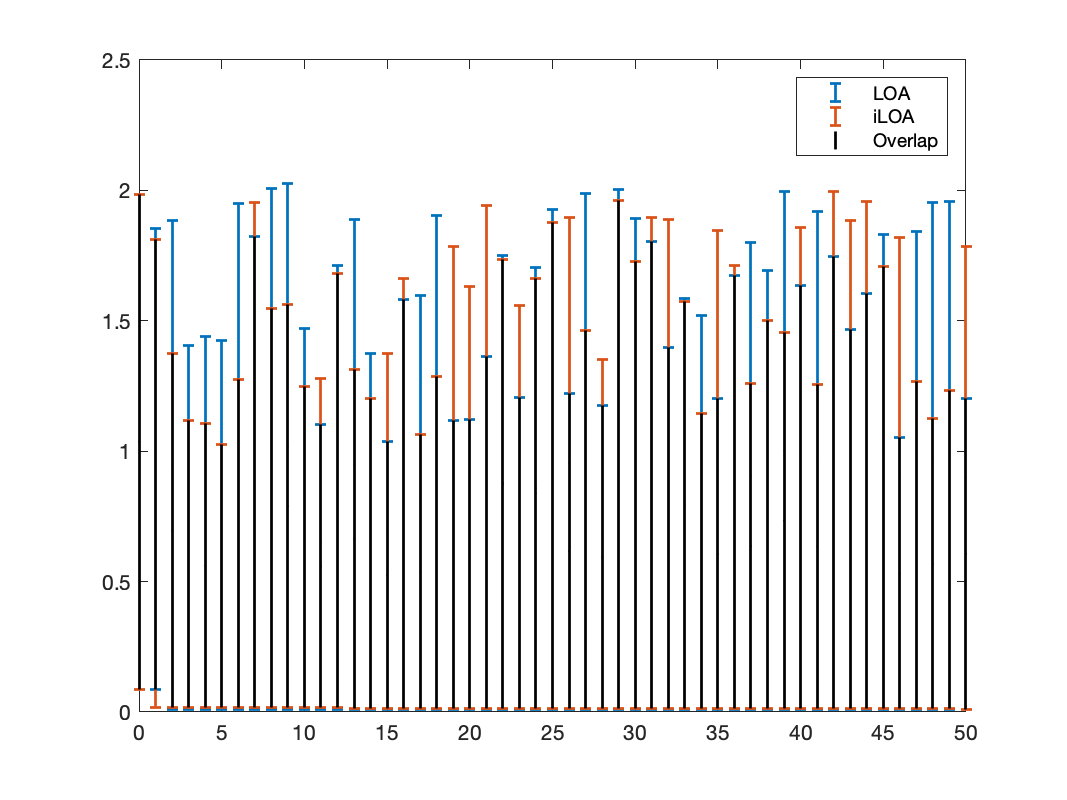
\includegraphics[width=\textwidth]{img/bars/f5/1}
    \caption{ \scriptsize Trial 1: Fitness Range (y) over Iterations (x)}
    \label{fig:f5-b-1}
  \end{subfigure}
  \begin{subfigure}[b]{0.4\textwidth}
    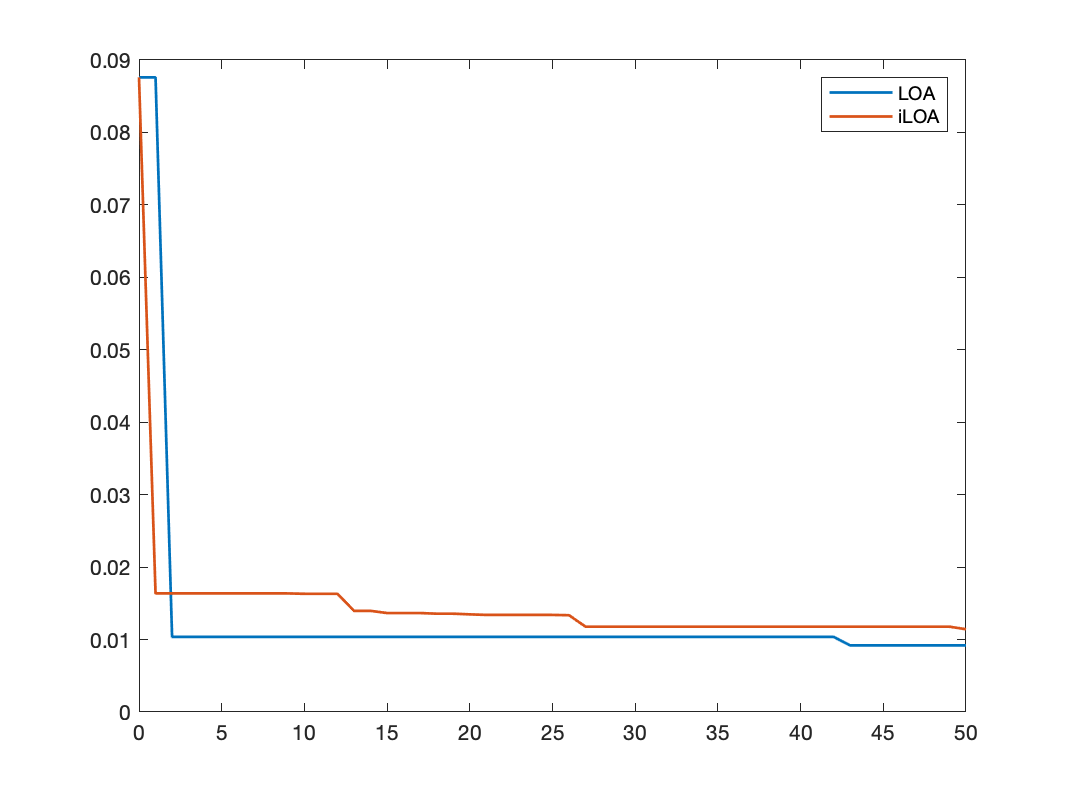
\includegraphics[width=\textwidth]{img/fits/f5/1}
    \caption{ \scriptsize Trial 1: Minimum Fitness (y) over Iterations (x)}
    \label{fig:f5-f-1}
  \end{subfigure}

  \begin{subfigure}[b]{0.4\textwidth}
    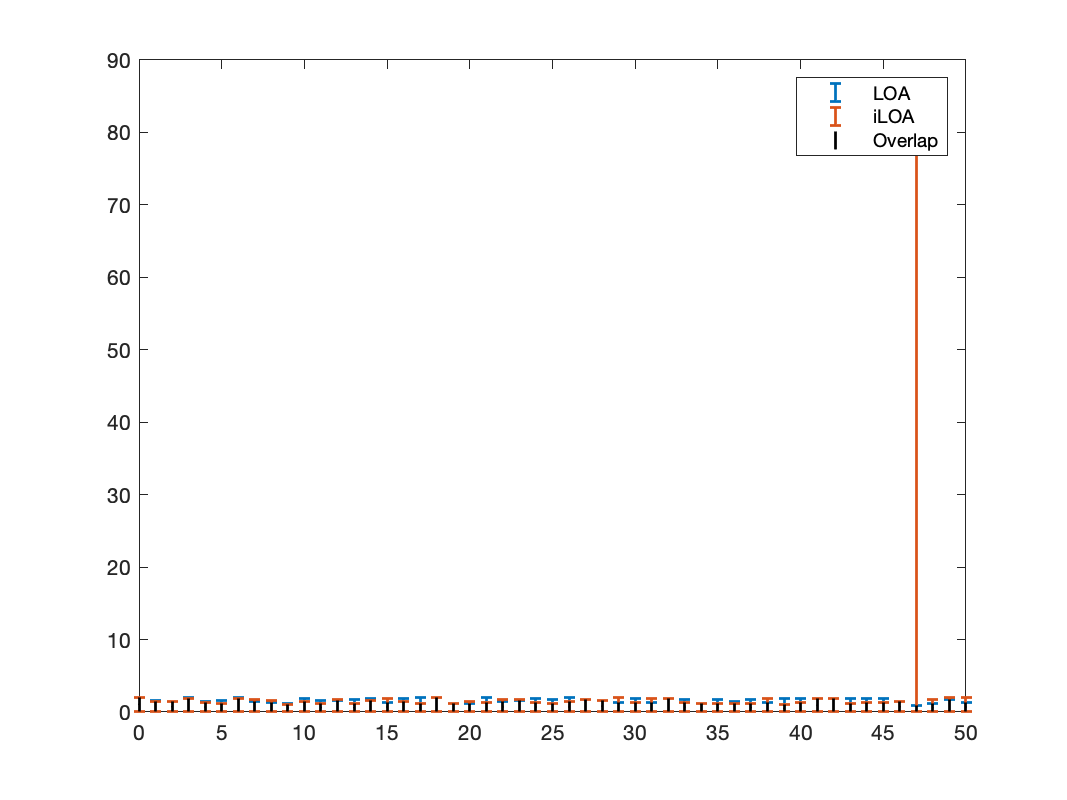
\includegraphics[width=\textwidth]{img/bars/f5/2}
    \caption{ \scriptsize Trial 2: Fitness Range (y) over Iterations (x)}
    \label{fig:f5-b-2}
  \end{subfigure}
  \begin{subfigure}[b]{0.4\textwidth}
    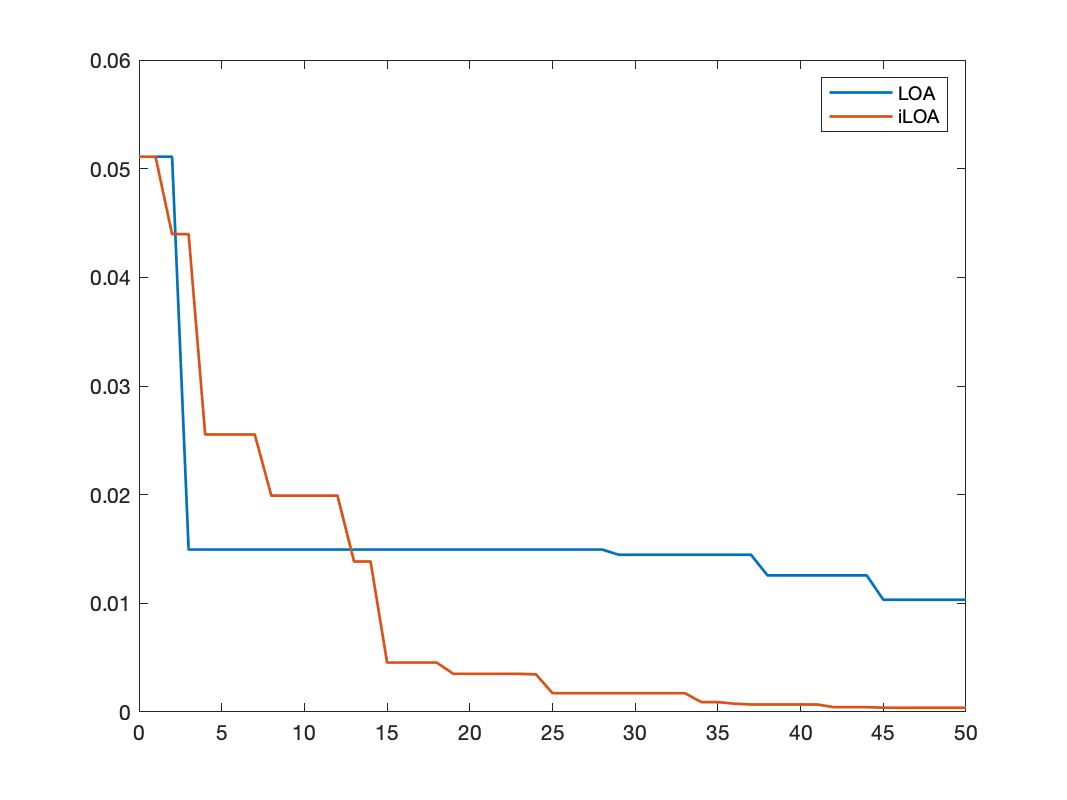
\includegraphics[width=\textwidth]{img/fits/f5/2}
    \caption{ \scriptsize Trial 2: Minimum Fitness (y) over Iterations (x)}
    \label{fig:f5-f-2}
  \end{subfigure}

  \begin{subfigure}[b]{0.4\textwidth}
    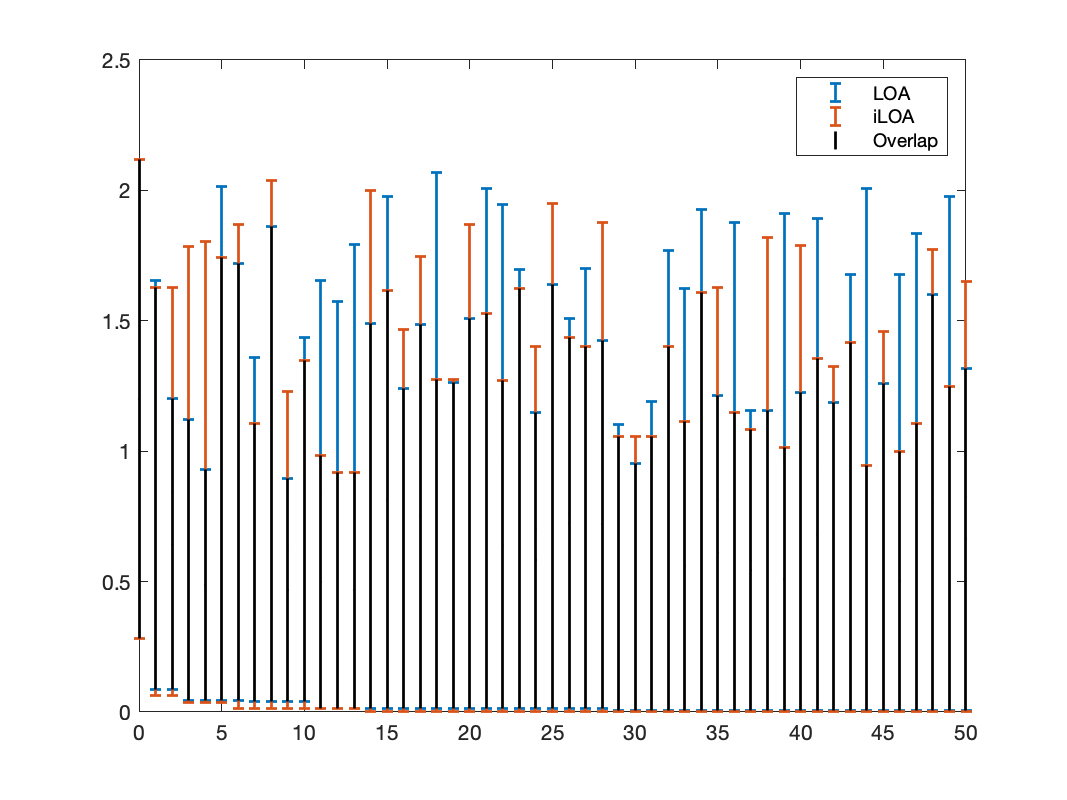
\includegraphics[width=\textwidth]{img/bars/f5/3}
    \caption{ \scriptsize Trial 3: Fitness Range (y) over Iterations (x)}
    \label{fig:f5-b-3}
  \end{subfigure}
  \begin{subfigure}[b]{0.4\textwidth}
    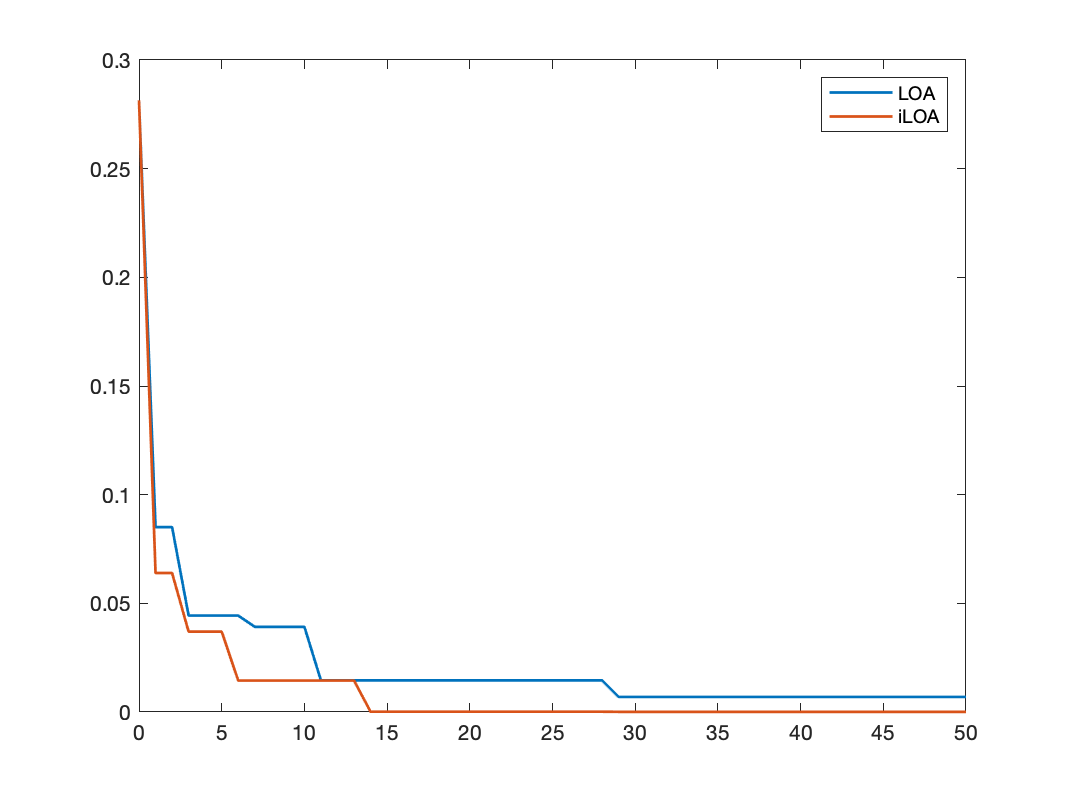
\includegraphics[width=\textwidth]{img/fits/f5/3}
    \caption{ \scriptsize Trial 3: Minimum Fitness (y) over Iterations (x)}
    \label{fig:f5-f-3}
  \end{subfigure}

  \begin{subfigure}[b]{0.4\textwidth}
    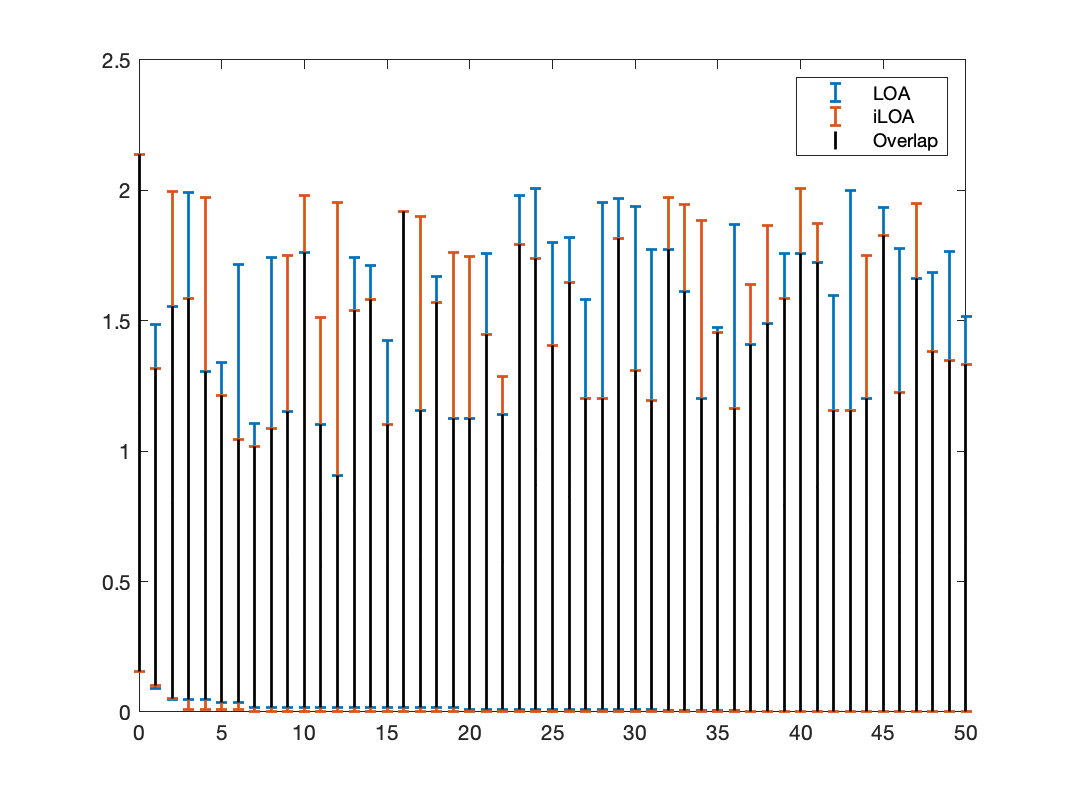
\includegraphics[width=\textwidth]{img/bars/f5/4}
    \caption{ \scriptsize Trial 4: Fitness Range (y) over Iterations (x)}
    \label{fig:f5-b-4}
  \end{subfigure}
  \begin{subfigure}[b]{0.4\textwidth}
    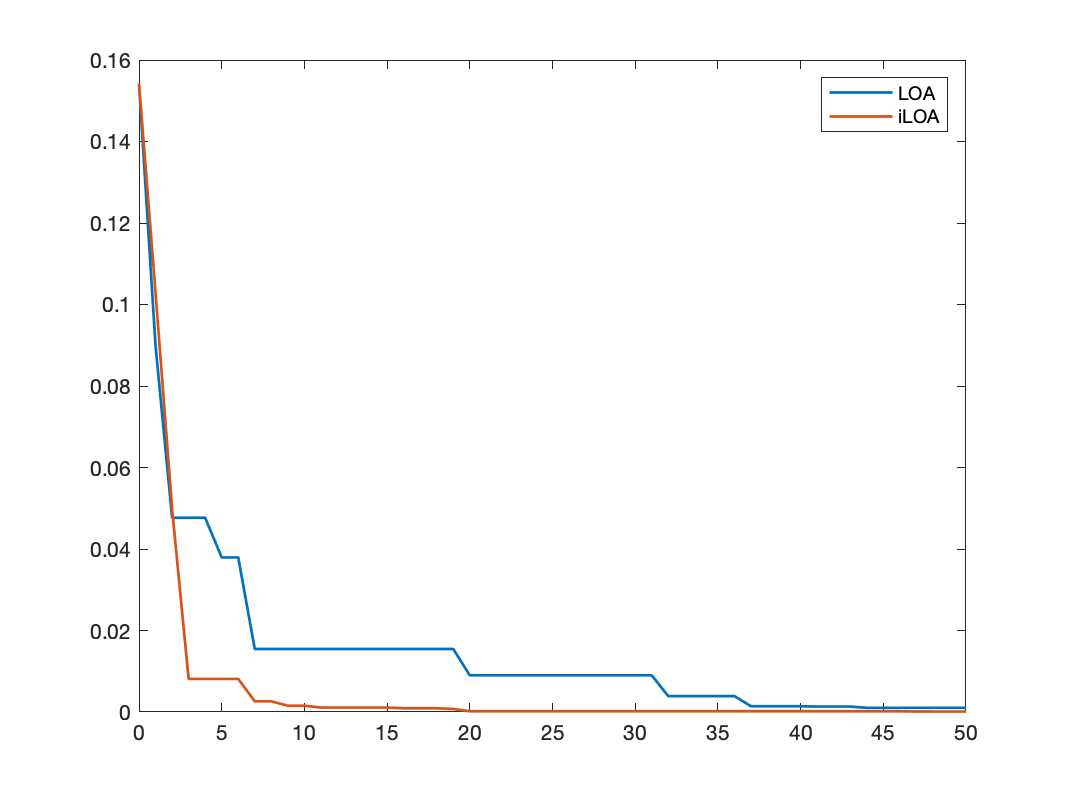
\includegraphics[width=\textwidth]{img/fits/f5/4}
    \caption{ \scriptsize Trial 4: Minimum Fitness (y) over Iterations (x)}
    \label{fig:f5-f-4}
  \end{subfigure}

  \begin{subfigure}[b]{0.4\textwidth}
    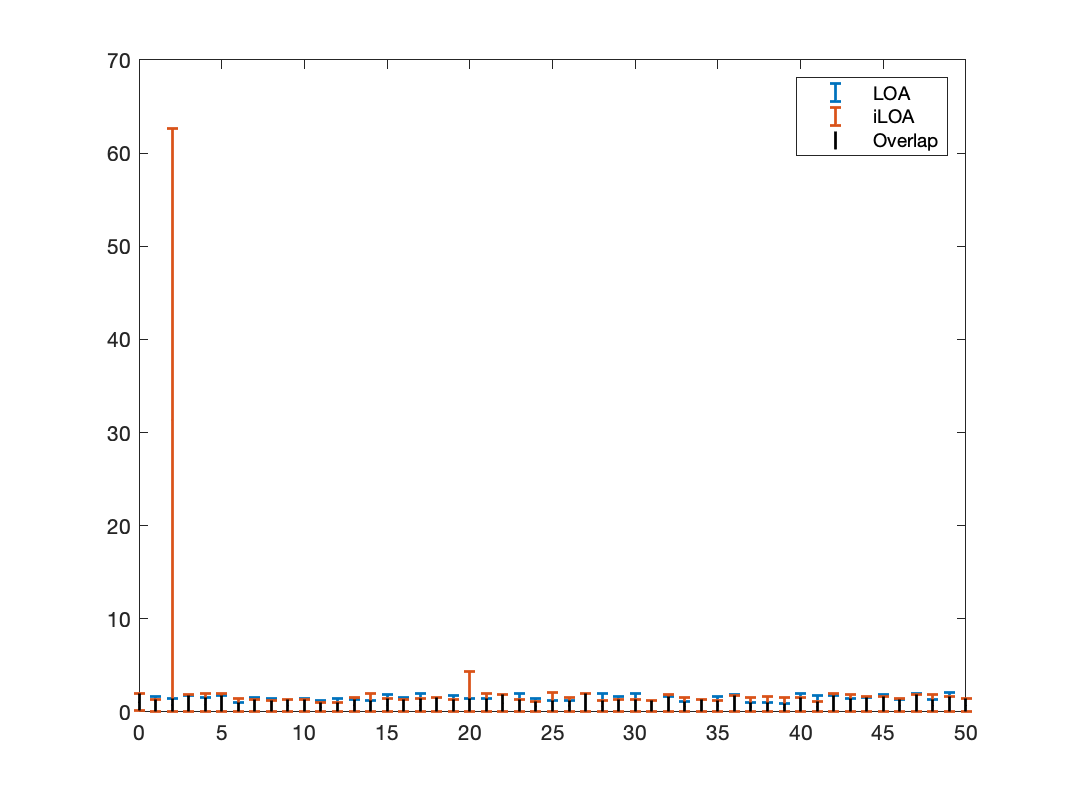
\includegraphics[width=\textwidth]{img/bars/f5/5}
    \caption{ \scriptsize Trial 5: Fitness Range (y) over Iterations (x)}
    \label{fig:f5-b-5}
  \end{subfigure}
  \begin{subfigure}[b]{0.4\textwidth}
    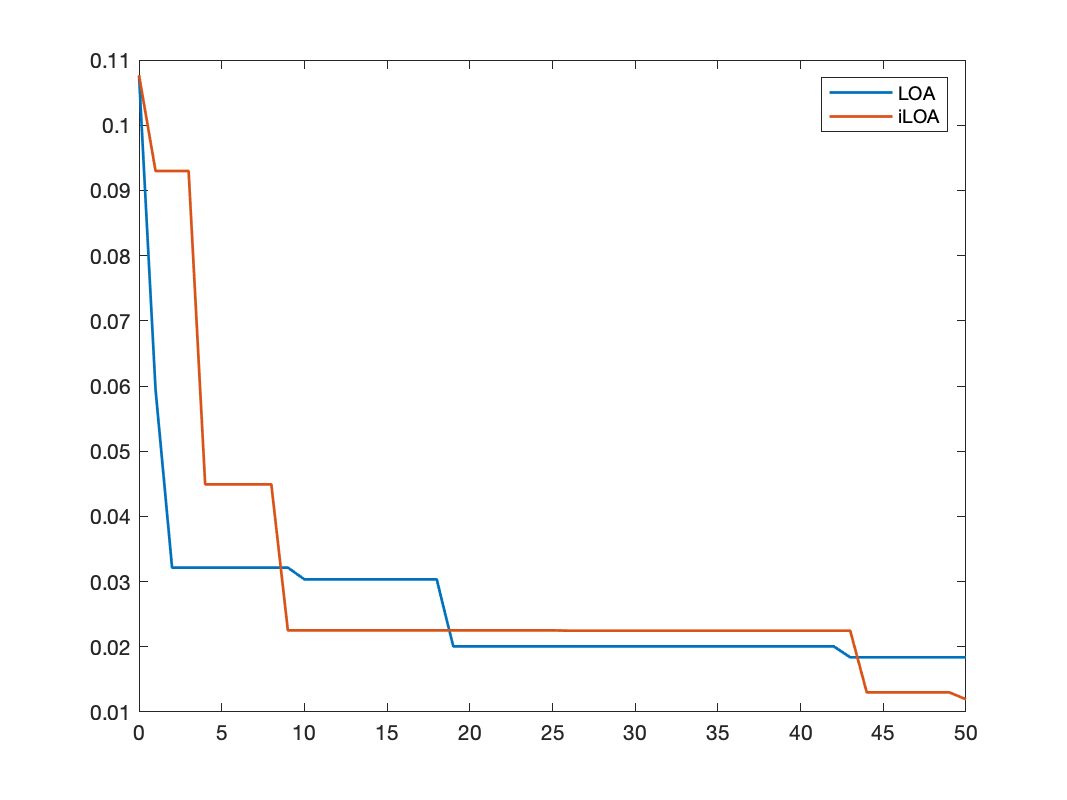
\includegraphics[width=\textwidth]{img/fits/f5/5}
    \caption{ \scriptsize Trial 5: Minimum Fitness (y) over Iterations (x)}
    \label{fig:f5-f-5}
  \end{subfigure}

  \caption{ \scriptsize LOA vs. iLOA: Rosenbrock 2D ($f_5$)}
\end{figure}
